%=======================================================================
%  Sensor-Aware Hypothesis Bank for Passive Frequency-Hopping
%  Generator Identification, Prediction and Response
%  IEEE conference paper (IEEEtran, two-column). Target: <= 6 pages.
%  Figures in figures/, numbers from results/ and docs/paper/ieee/data/.
%=======================================================================
\documentclass[conference]{IEEEtran}
\IEEEoverridecommandlockouts
\usepackage{cite}
\usepackage{amsmath,amssymb,amsfonts}
\usepackage{algorithm}
\usepackage{algorithmic}
\usepackage{graphicx}
\usepackage{textcomp}
\usepackage{booktabs}
\usepackage{multirow}
\usepackage{xcolor}
\usepackage{array}
\usepackage{stfloats}
\graphicspath{{figures/}}
% Tighter float spacing to hold the page budget.
\setlength{\textfloatsep}{9pt plus 2pt minus 2pt}
\setlength{\dbltextfloatsep}{9pt plus 2pt minus 2pt}
\setlength{\floatsep}{7pt plus 2pt minus 2pt}
\def\BibTeX{{\rm B\kern-.05em{\sc i\kern-.025em b}\kern-.08em
    T\kern-.1667em\lower.7ex\hbox{E}\kern-.125emX}}

\begin{document}

\title{Sensor-Aware Passive Frequency-Hopping Prediction and
Generator Identification for Electronic Warfare}

\author{
\IEEEauthorblockN{
Md. Rifatuddin Romel\IEEEauthorrefmark{1},
Rashad Zaki Raiyan,
Abdullah Ahnaf Karim,
Saiyara Sabah,
Arif Aziz
}
\IEEEauthorblockA{\textit{Officer's Training School, Bangladesh Air Force} \\
Jashore, Bangladesh \\
\IEEEauthorrefmark{1}Corresponding author: rifatuddin443@gmail.com}
}
\maketitle
\begin{abstract}
Modern radios hop under many different algorithms, so a passive
electronic-support receiver must work out, in a short engagement window and
through a lossy sensor, which generator drives a frequency-hopping (FH) emitter
and which channel comes next, or it cannot protect the spectrum it monitors. We
present FHBP, which reduces the sensor's misses and false alarms to one
detection-level likelihood per slot and scores a bank of known generators with
it. FHBP locks onto a generator once it holds more than $95\%$ of the posterior
probability, or under an anytime-valid stopping rule. The same likelihood
drives a training-free next-channel predictor, a change-point tracker for
mid-engagement generator switches, and a conformal prediction set with a
distribution-free coverage guarantee. Across more than $15{,}000$ simulated
episodes (thirteen generators, four sensor operating points), deterministic
in-bank families, except a full-state LCG whose period is too short at
$M{=}16$, are identified at $\geq 0.96$ accuracy even on a contested sensor
($P_d{=}0.6$). False algebraic identifications stay at or below $0.05$, while a
closed-set test makes them on $0.24$ of out-of-bank emitters. On held-out
generators, prediction reaches $1.00$ top-1 where an LSTM falls to $0.09$, and
conformal sets hold $\geq 0.90$ coverage where a fixed shortlist covers as
little as $0.19$. Hops-to-identify is within $1.3$--$2.7\times$ an
information-theoretic lower bound, and one slot costs about $3$\,ms on one CPU
core ($46$\,ms with switch tracking).
\end{abstract}

\begin{IEEEkeywords}
frequency hopping, electronic support, sequential hypothesis testing,
online prediction, conformal prediction, change-point detection.
\end{IEEEkeywords}

%=======================================================================
\section{Introduction}
%=======================================================================
Frequency hopping (FH) is used to  resist interception
and jamming in radio links: the carrier frequency changes from slot to slot under the control
of a pseudo-random generator. A passive electronic-support (ES) receiver that
wants to characterise such emitter has to answer three questions- generator algorithm in use and frequency hopped to next. Most existing methods answer one of these questions and assume a clean stream. Besides, finding how predictable the emitter is in the first place also matters
because a keyed cryptographic generator is designed to look like noise, and the
receiver should report it as such instead of forcing a match, which is not available in literature to the best of our knowledge. All these answers
are needed within fewest hops, through an imperfect sensor


Neural predictors forecast the next hop of one specific family from an
idealised stream~\cite{li2020lstm,li2021china,zhu2023recovery,basak2024spectrum}.
Sequential detectors identify a parameter, but do not choose among different
kinds of generator family~\cite{baum1994,dragalin1999}. Particle filters track
a hopped carrier but not the \emph{algorithm} behind
it~\cite{valyrakis2009,sidiropoulos2006}. None scores a bank of competing
generator families through an explicit sensor model, and none couples a
calibrated forecast to a decision with a stated guarantee.

This paper presents FHBP, which predicts the class of generator first to predict the future hop sequence. This eliminates the need for prior training that is required by ML/DL models. It also reduce the lossy passive sensor to a single per-slot
\emph{detection-level likelihood}, set only by the detection and false-alarm
probabilities $(P_d,P_{fa})$, and use that one quantity at every stage:
identification, stopping, prediction, change tracking and response. Because
every stage reads the same quantity, a mixed bank of unrelated generators,
classical recovery attacks and a distribution-free guarantee all run inside one
loop. Each contribution is backed by a simulation under an \emph{information-parity}
rule: every expert and baseline sees only the sensor's detections, never the
true channel sequence or the generator instance.

\begin{enumerate}
\item \textbf{A unified sensor-aware hypothesis bank.} One $(P_d,P_{fa})$
likelihood scores different
generator classes, plus an explicit generative none-of-the-above class $H_0$, with
MSPRT or an anytime-valid e-process for stopping (Sec.~\ref{sec:bank}). No
prior passive-FH method scores a bank of competing generator families through
one detection-level likelihood. Without the $H_0$ (“unknown”) option, $24\%$ of unfamiliar emitters are misidentified as algebraic generators; with it, false identifications stay at or below $5\%$ on every sensor.

\item \textbf{A training-free predictor that generalises beyond the bank.}
A Fixed-Share mixture of the bank's experts and an always-on, training-free
universal expert keeps predicting hops even for generators the bank does
not contain (Sec.~\ref{sec:predict}). On a held-out generator it reaches
$1.00$ steady-state top-1 accuracy, versus $0.38$ for identification alone
and $0.09$ for an LSTM trained on the bank's families; on a keyed
cryptographic generator it correctly falls to chance.
\item \textbf{A change-point tracker over the generator.} A Bayesian online
change-point posterior whose run-length hypotheses each carry a
\emph{switch-anchored} bank detects, dates and re-identifies a mid-engagement
change of the generating algorithm from the lossy stream (Sec.~\ref{sec:switch}).
Prior FH change-point work handles hop-timing transients, not a change of the
generator itself.

\item \textbf{A conformal set tied to the response.} The set grows or shrinks
online to hold a distribution-free coverage level (Sec.~\ref{sec:conformal}).
Because the set is the multi-tone jam plan, that coverage becomes a
``fraction-of-hops-denied'' guarantee. A fixed shortlist covers as little as
$0.19$ on an unpredictable source; the conformal set holds $\geq 0.90$ by
adjusting its size, so the data sets the tone count.
\end{enumerate}

We test on thirteen generators at four sensor operating points against
conventional identifiers and external predictors on the same episodes, add a
mis-specified-sensor stress test, measure per-slot compute and compare
hops-to-identify against an information-theoretic converse.
%=======================================================================
\section{Related Work}
%=======================================================================
OTS sits at the meeting of four lines that have matured largely apart:
learned prediction and recovery of hopping sequences, sequential detection
with sensor-aware likelihoods, online/anytime-valid uncertainty
quantification, and the predictive-jamming loop that consumes a forecast.
We review each and state the gap it leaves.

\textbf{FH prediction and recovery.} Learned next-hop prediction is an
established task. LSTM models forecast non-cooperative FH frequencies from
intercepted data~\cite{li2020lstm,li2021china}; a CNN--GRU recovers sequences
with transfer learning across hop-sets~\cite{zhu2023recovery}; a CNN--LSTM
predicts drone FHSS occupancy on real
signals~\cite{basak2024spectrum}; and recent entries add a TCN--GRU with
Bayesian optimisation~\cite{zhong2024tcngru}, a Transformer over phase-space
reconstructed chaotic hops~\cite{cao2025transformer}, and a homotopy-HMM for
nonlinear hops under scarce priors~\cite{deng2025hthmm}. All are trained or
tuned per family on largely clean time--frequency data and emit a point
prediction. The closest ``identify, predict, flag unknown'' precedent
reverse-engineers LFSR hoppers with a neural
network~\cite{strickland2023}, but is LFSR-only, trained, and clean-data. On
the algebraic side, recovery of a specific mechanism is classical and sharp:
Berlekamp--Massey for LFSRs~\cite{massey1969}, and lattice/seed-search methods
for congruential and weakly-keyed generators~\cite{reeds1977}; these degrade
abruptly under missed detections. Separately, transformers have been shown to
predict linear-congruential outputs in context~\cite{tao2025transformers}, and
a follow-up extends this to permuted congruential generators under
truncation~\cite{tao2026pcg}---the sharpest precedent for ``predict without
knowing the generator'', though it requires large-scale pretraining. OTS
differs by being training-free and online, scored under an explicit
$(P_d,P_{fa})$ sensor, and tied to an identification bank rather than run as a
standalone forecaster.

\textbf{Sequential tests and sensor likelihoods.} Our threshold rule is the
MSPRT of~\cite{baum1994}, optimal under correlated (HMM)
observations~\cite{dragalin1999}; the e-process is a safe anytime-valid
test~\cite{ramdas2023}, and the matching nonparametric change framework is the
e-detector of~\cite{shin2023edetectors}. The generative $H_0$ follows the
no-match idea of~\cite{gutman1989}. The reduced emission is the
discrete-channel form of the detection/clutter likelihood behind probabilistic
data association~\cite{barshalom2009}; cognitive-radio spectrum prediction
likewise folds $P_d/P_{fa}$ into HMM emissions. Particle filters track a hopped
\emph{carrier}~\cite{valyrakis2009,sidiropoulos2006} but not the algorithm
behind it. These supply every component, but none runs \emph{one} shared
detection-level likelihood across a bank of competing generator families, which
is the assembly OTS contributes.

\textbf{The predictive-jamming loop.} Acting on a predicted channel is the dual
problem. Deployed Bluetooth hop-prediction attacks infer the hopping behaviour
of an undiscoverable link and act on it~\cite{blueear2016}; learned anti-jamming
hopping is the defender's side~\cite{qi2024drl}; and predictive/learning jammers
that follow or jam the predicted channel exist, including DRL resource
allocation against FHSS~\cite{rao2024sensors} and a recent risk-constrained
adaptive hopper that reasons about a predictive jammer's exposure of
high-probability channels~\cite{chen2026risk}. None self-identifies the
generator first, and none sizes the response from the \emph{entropy} of a
calibrated next-hop distribution. We treat the multi-tone response only as a
downstream use of the calibrated forecast, not as a new jammer, and compare
against a reactive-follower floor rather than claiming a first predictive
attack.


%=======================================================================
\section{System Model and Methodology}
\label{sec:method}
%=======================================================================
Fig.~\ref{fig:arch} shows the end-to-end data flow and
Algorithm~\ref{alg:loop} the per-slot loop.

\begin{figure}[t]
\centering
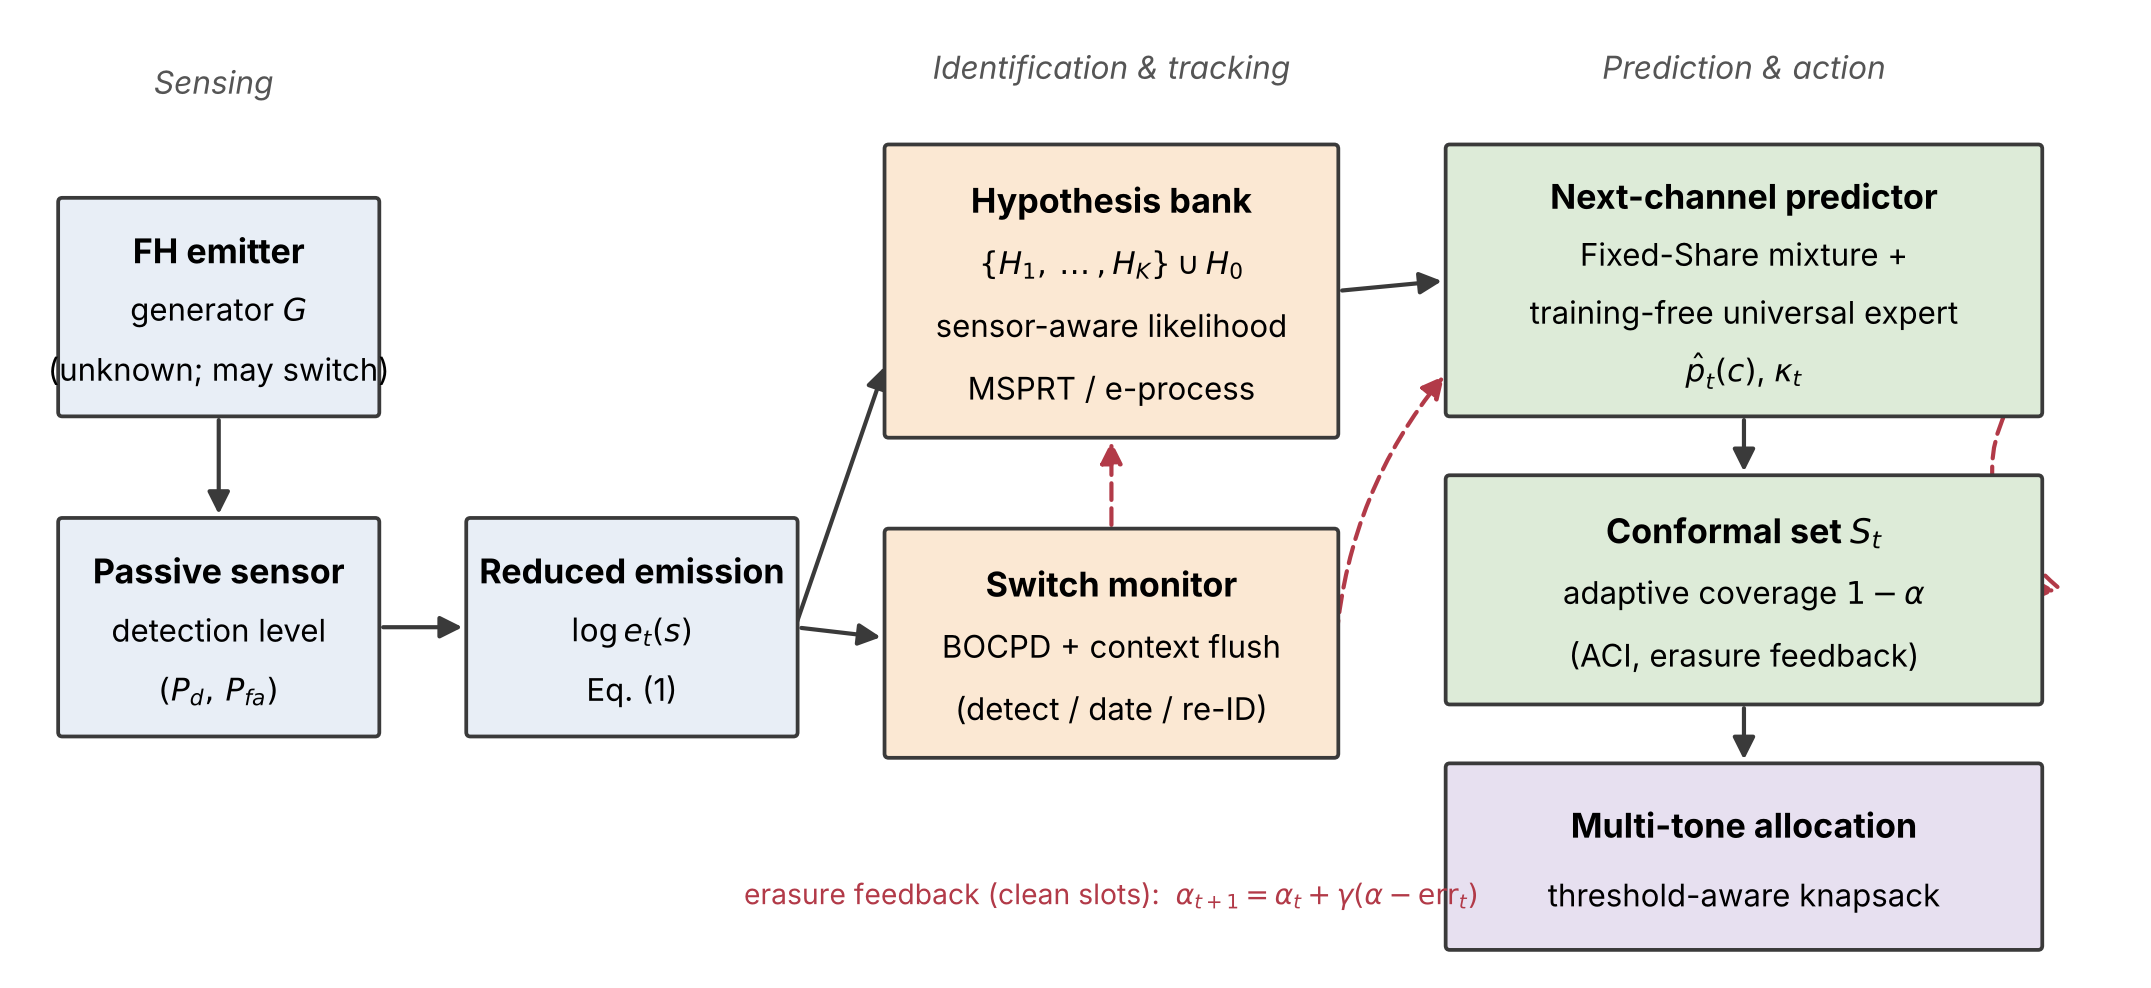
\includegraphics[width=0.9\columnwidth]{fig_architecture.png}
\caption{System architecture. One detection-level likelihood feeds the
hypothesis bank, the switch monitor, the next-channel predictor and the
conformal set; the set drives the multi-tone response. Dashed red: the switch
monitor resets the bank/predictor, and erasure feedback calibrates the
conformal level online.}
\label{fig:arch}
\end{figure}

\subsection{Problem and sensor model}
A single emitter transmits, at slot $t=1,\dots,T$, on channel $c_t$ from a set
$C$ of size $M$ (default $M=16$). The channel is chosen by an unknown generator
$G$. A passive sensor detects the true channel with probability $P_d$. On every
other channel it raises an independent false alarm with probability $P_{fa}$.
The result is a detection set $D_t\subseteq C$. For a hypothesised true channel
$s$, we factor out the all-false-alarm constant $F_t$, which is the same for
every hypothesis. What remains is the \emph{reduced emission}
\begin{equation}
\log e_t(s)=
\begin{cases}
\log(P_d/P_{fa}), & s\in D_t,\\[2pt]
\log\!\big((1-P_d)/(1-P_{fa})\big), & s\notin D_t.
\end{cases}
\label{eq:emit}
\end{equation}
$F_t$ cancels in every posterior and likelihood ratio, so the whole system
works with \eqref{eq:emit}. The equation is used twice: once to generate
observations and once inside every expert. Because the same simulator both
generates adversaries and scores them, we enforce \emph{information parity}. An
expert sees only the stream of observations and its own bounded reconnaissance
ranges. It never sees the true channel sequence or the generator instance.

\subsection{The hypothesis bank and stopping rules}
\label{sec:bank}
The bank keeps a posterior over $\{H_0,H_1,\dots,H_K\}$. After every slot it
updates the posterior with each expert's reduced likelihood,
$\pi_t(k)\propto\pi_{t-1}(k)\,P(o_t\mid o_{1:t-1},H_k)$. A floor on the $H_0$
prior means the unknown class is never ruled out. Deterministic families
(LFSR, filtered LFSR, LCG, weak-seed) are handled by a particle filter over
the family's parameter space. Each candidate parameterisation is one particle,
and its deterministic trajectory is scored through \eqref{eq:emit}. This
scoring is immune to gaps because it never needs consecutive outputs. Markov
and chaotic families use a channel-level HMM forward pass.

Two stopping rules read the cumulative reduced log-likelihoods. \emph{MSPRT}
declares $k^\ast=\arg\max_k\pi_t(k)$ when $\pi_t(k^\ast)\geq1-\delta$;
$k^\ast=0$ means \emph{unknown}. The \emph{e-process} declares $k$ when the
e-value against its strongest competitor,
$E_t(k)=P(o_{1:t}\mid H_k)/\max_{j\neq k}P(o_{1:t}\mid H_j)$, crosses $1/\beta$.
By Ville's inequality, this bounds the probability of ever declaring a wrong
in-bank $k$ by $\beta$ per competitor.

\subsection{Next-channel prediction}
\label{sec:predict}
Naming the generator is only a step towards the output an operator needs, which
is the next channel. A Fixed-Share expert mixture weights
experts by their \emph{recent} one-step predictive skill,
\begin{equation}
w_{t+1}(i)\propto w_t(i)\,e^{\eta\,\ell_t(i)},\quad
w_{t+1}\leftarrow(1-\alpha)w_{t+1}+\alpha/N,
\end{equation}
and mixes their forecasts, $\hat p_t(c)=\sum_i w_t(i)\,p_i(c)$. The share floor
$\alpha$ lets a dormant expert recover after a change. The mixture always
carries a \emph{training-free universal} expert, a gap-robust variable-order
context-mixing model. When no identification expert fits a new generator, the
universal expert gains weight and carries the forecast, so the mixture does
not collapse to the uniform floor. The system also reports the predictability
score $\kappa_t=1-H(\hat p_t)/\log M$.

\subsection{Switch tracking}
\label{sec:switch}
An identifier that accumulates evidence is slow to forget it. We therefore run
a Bayesian online change-point posterior in which each run-length hypothesis
carries its own bank, \emph{anchored at the hypothesised switch slot}. A
freshly re-keyed or counter-based generator can then restart from zero, and
one posterior detects, dates, re-identifies and predicts at the same time. A
cheaper CUSUM monitor watches the mixture's loss stream. On an alarm it resets
the Fixed-Share weights and flushes the universal predictor's stale context.

\subsection{Conformal sets and response}
\label{sec:conformal}
A point forecast carries no guarantee. We therefore emit a prediction set
$S_t$: the smallest top-ranked set whose predictive mass reaches an online
level $1-\alpha_t$. The level $\alpha_t$ is updated by Adaptive Conformal
Inference~\cite{gibbs2021},
$\alpha_{t+1}=\mathrm{clip}(\alpha_t+\gamma(\alpha-\mathrm{err}_t),0,1)$. The
calibration signal $\mathrm{err}_t$ is the erasure feedback a passive node
actually receives (clean slots only), so coverage holds over the clean
sub-stream without assuming exchangeability. The set \emph{is} the multi-tone
jam plan. Funding every channel in $S_t$ denies the realised next hop at the
coverage rate, so the fraction of hops denied inherits the distribution-free
$1-\alpha$ bound. The underlying allocator is a threshold-aware greedy
knapsack: it ranks channels by predicted mass per unit denial cost and funds
them up to a budget.

\begin{algorithm}[t]
\caption{Engagement loop (one emitter, window $T$)}
\label{alg:loop}
\begin{algorithmic}
\STATE $\pi\leftarrow\pi_0$; reset every expert
\FOR{$t=1$ \TO $T$}
  \STATE $o_t\leftarrow\mathrm{observe}()$; form $\log e_t$ by \eqref{eq:emit}
  \FOR{$k=0$ \TO $K$}
     \STATE $\ell_k\leftarrow H_k.\mathrm{step}(\log e_t)$;\;
            $\Lambda(k)\mathrel{+}=\ell_k$;\; $H_k.\mathrm{observe\_clean}(o_t)$
  \ENDFOR
  \STATE $\pi\leftarrow\mathrm{softmax}(\log\pi_0+\Lambda)$
  \STATE $\hat p\leftarrow$ Fixed-Share predictor; form set $S_t$
  \IF{stop rule fires}
     \STATE \textbf{return} declare$(\arg\max_k\pi)$, $\tau=t$
  \ENDIF
\ENDFOR
\STATE \textbf{return} declare$(\arg\max_k\pi)$, $\tau=T$
\end{algorithmic}
\end{algorithm}

%=======================================================================
\section{Experimental Setup}
\label{sec:setup}
%=======================================================================
All experiments are simulation-only with $M=16$ and fixed seeds, and every
figure is regenerated from saved JSON. Table~\ref{tab:gens} lists the generator
library. Three ``held-out'' families (lagged Fibonacci, quadratic congruential,
sine map) have \emph{no} dedicated expert, so they test whether prediction
generalises. A keyed SHA-256 CSPRNG is the unpredictable control. We sweep four
sensor operating points: Perfect $(1.0,0)$, Strong $(0.95,0.01)$, Typical
$(0.8,0.02)$ and Contested $(0.6,0.05)$. Identification uses MSPRT with
$\delta=0.05$. We report three identification measures: accuracy,
hops-to-identify $\tau$, and the \emph{hard} false-ID rate. A hard false ID is
the dangerous error of declaring an algebraic family (LFSR, filtered LFSR, LCG,
weak-seed) that is not the truth. Prediction is scored by steady-state top-1
next-channel accuracy against the chance line $1/M=0.0625$. The headline
identification evaluation aggregates $100$ seeds $\times$ $13$ generators
$\times$ $4$ sensors ($5{,}200$ episodes). The coverage experiment adds
$7{,}500$, and the identifier-baseline, predictor-baseline and response
experiments below add $2{,}000$, $450$ and $540$, for $15{,}690$ in total.

\emph{Baselines} see the same episodes through the same sensor. For
identification we use three: a pairwise SPRT and a fixed-length ($30$-hop)
likelihood-ratio test, both over the \emph{same} experts and likelihood
\eqref{eq:emit} but without $H_0$; and a feature classifier with an
\emph{unknown} class, trained on $2{,}100$ simulated episodes from the bank's
parameter ranges and deciding on the whole window. For prediction we also use
three: an online first-order Markov counter; online PPM-C (orders $0$--$4$);
and a two-layer, $128$-unit LSTM trained offline on $18{,}000$ sequences of the
six in-bank families at the test sensor (input: per-slot detection mask; label:
true next channel).

\begin{table}[t]
\centering
\caption{Generator library. Held-out families have no expert.}
\label{tab:gens}
\setlength{\tabcolsep}{4pt}
\footnotesize
\begin{tabular}{@{}lll@{}}
\toprule
Family & Structure & Hidden parameters \\
\midrule
LFSR / filt.\ LFSR & shift register ($+$ combiner) & taps, length, state \\
LCG / full LCG & $x\!\leftarrow\!(ax{+}c)\bmod m$ & $m,a,c,\text{seed}$ \\
weak-seed & small-keyspace PRNG & seed \\
Markov & first-order hopper & transition matrix \\
logistic/tent/H\'enon & chaotic maps, quantised & map parameter, $x_0$ \\
\midrule
lagged-Fib. (held out) & $c_t{=}(c_{t-1}{+}c_{t-k})\bmod M$ & order $k$ \\
quad.-CG (held out) & $x\!\leftarrow\!(ax^2{+}bx{+}c)\bmod M$ & $a,b,c$ \\
sine map (held out) & $x\!\leftarrow\!r\sin(\pi x)$ & $r,x_0$ \\
CSPRNG (control) & SHA-256 counter mode & key \\
\bottomrule
\end{tabular}
\end{table}

%=======================================================================
\section{Results}
\label{sec:results}
%=======================================================================

\subsection{Identification: coverage and safety}
Fig.~\ref{fig:confusion} shows family confusion matrices at the four sensors.
The diagonal is clean for every generator that an expert targets. As the sensor
degrades, the errors are safe ones: a held-out generator or a worn-down Markov
source is routed to the Markov or $H_0$ column, never to a false algebraic
claim. Table~\ref{tab:ident} aggregates the identifiable families.
Deterministic families are named at $\geq 0.99$ accuracy in a handful of hops
down to the typical sensor, and at $\geq 0.96$ on the contested one. The hard
false-ID rate stays at or below $0.05$ throughout. It is $0.00$ for the
shift-register and weak-seed families, which are the ones an operator would
most dangerously misattribute. The exception among deterministic families is
the full-state LCG. Its period at $M{=}16$ is at most $16$, and as the sensor
degrades the bank increasingly reads it as a Markov cycle
(Fig.~\ref{fig:confusion}, Sec.~\ref{sec:discussion}).

\emph{Against conventional identifiers.} Table~\ref{tab:idbase} runs the bank
and three baselines on identical episodes: the seven generators of
Table~\ref{tab:ident} plus the three held-out families. In-bank, the
closed-set tests are nearly as accurate as the bank, since they share its
likelihood. Out of bank they are forced to name something. The pairwise SPRT
names an algebraic generator on $0.88$ of CSPRNG episodes and $0.24$ of all
out-of-bank episodes, against $0.005$ for the bank. The learned classifier does
have an \emph{unknown} class, but it works from summary statistics, and under
those statistics congruential, weak-seed and keyed streams look alike. It is
therefore both less accurate and less safe.

\begin{figure}[t]
\centering
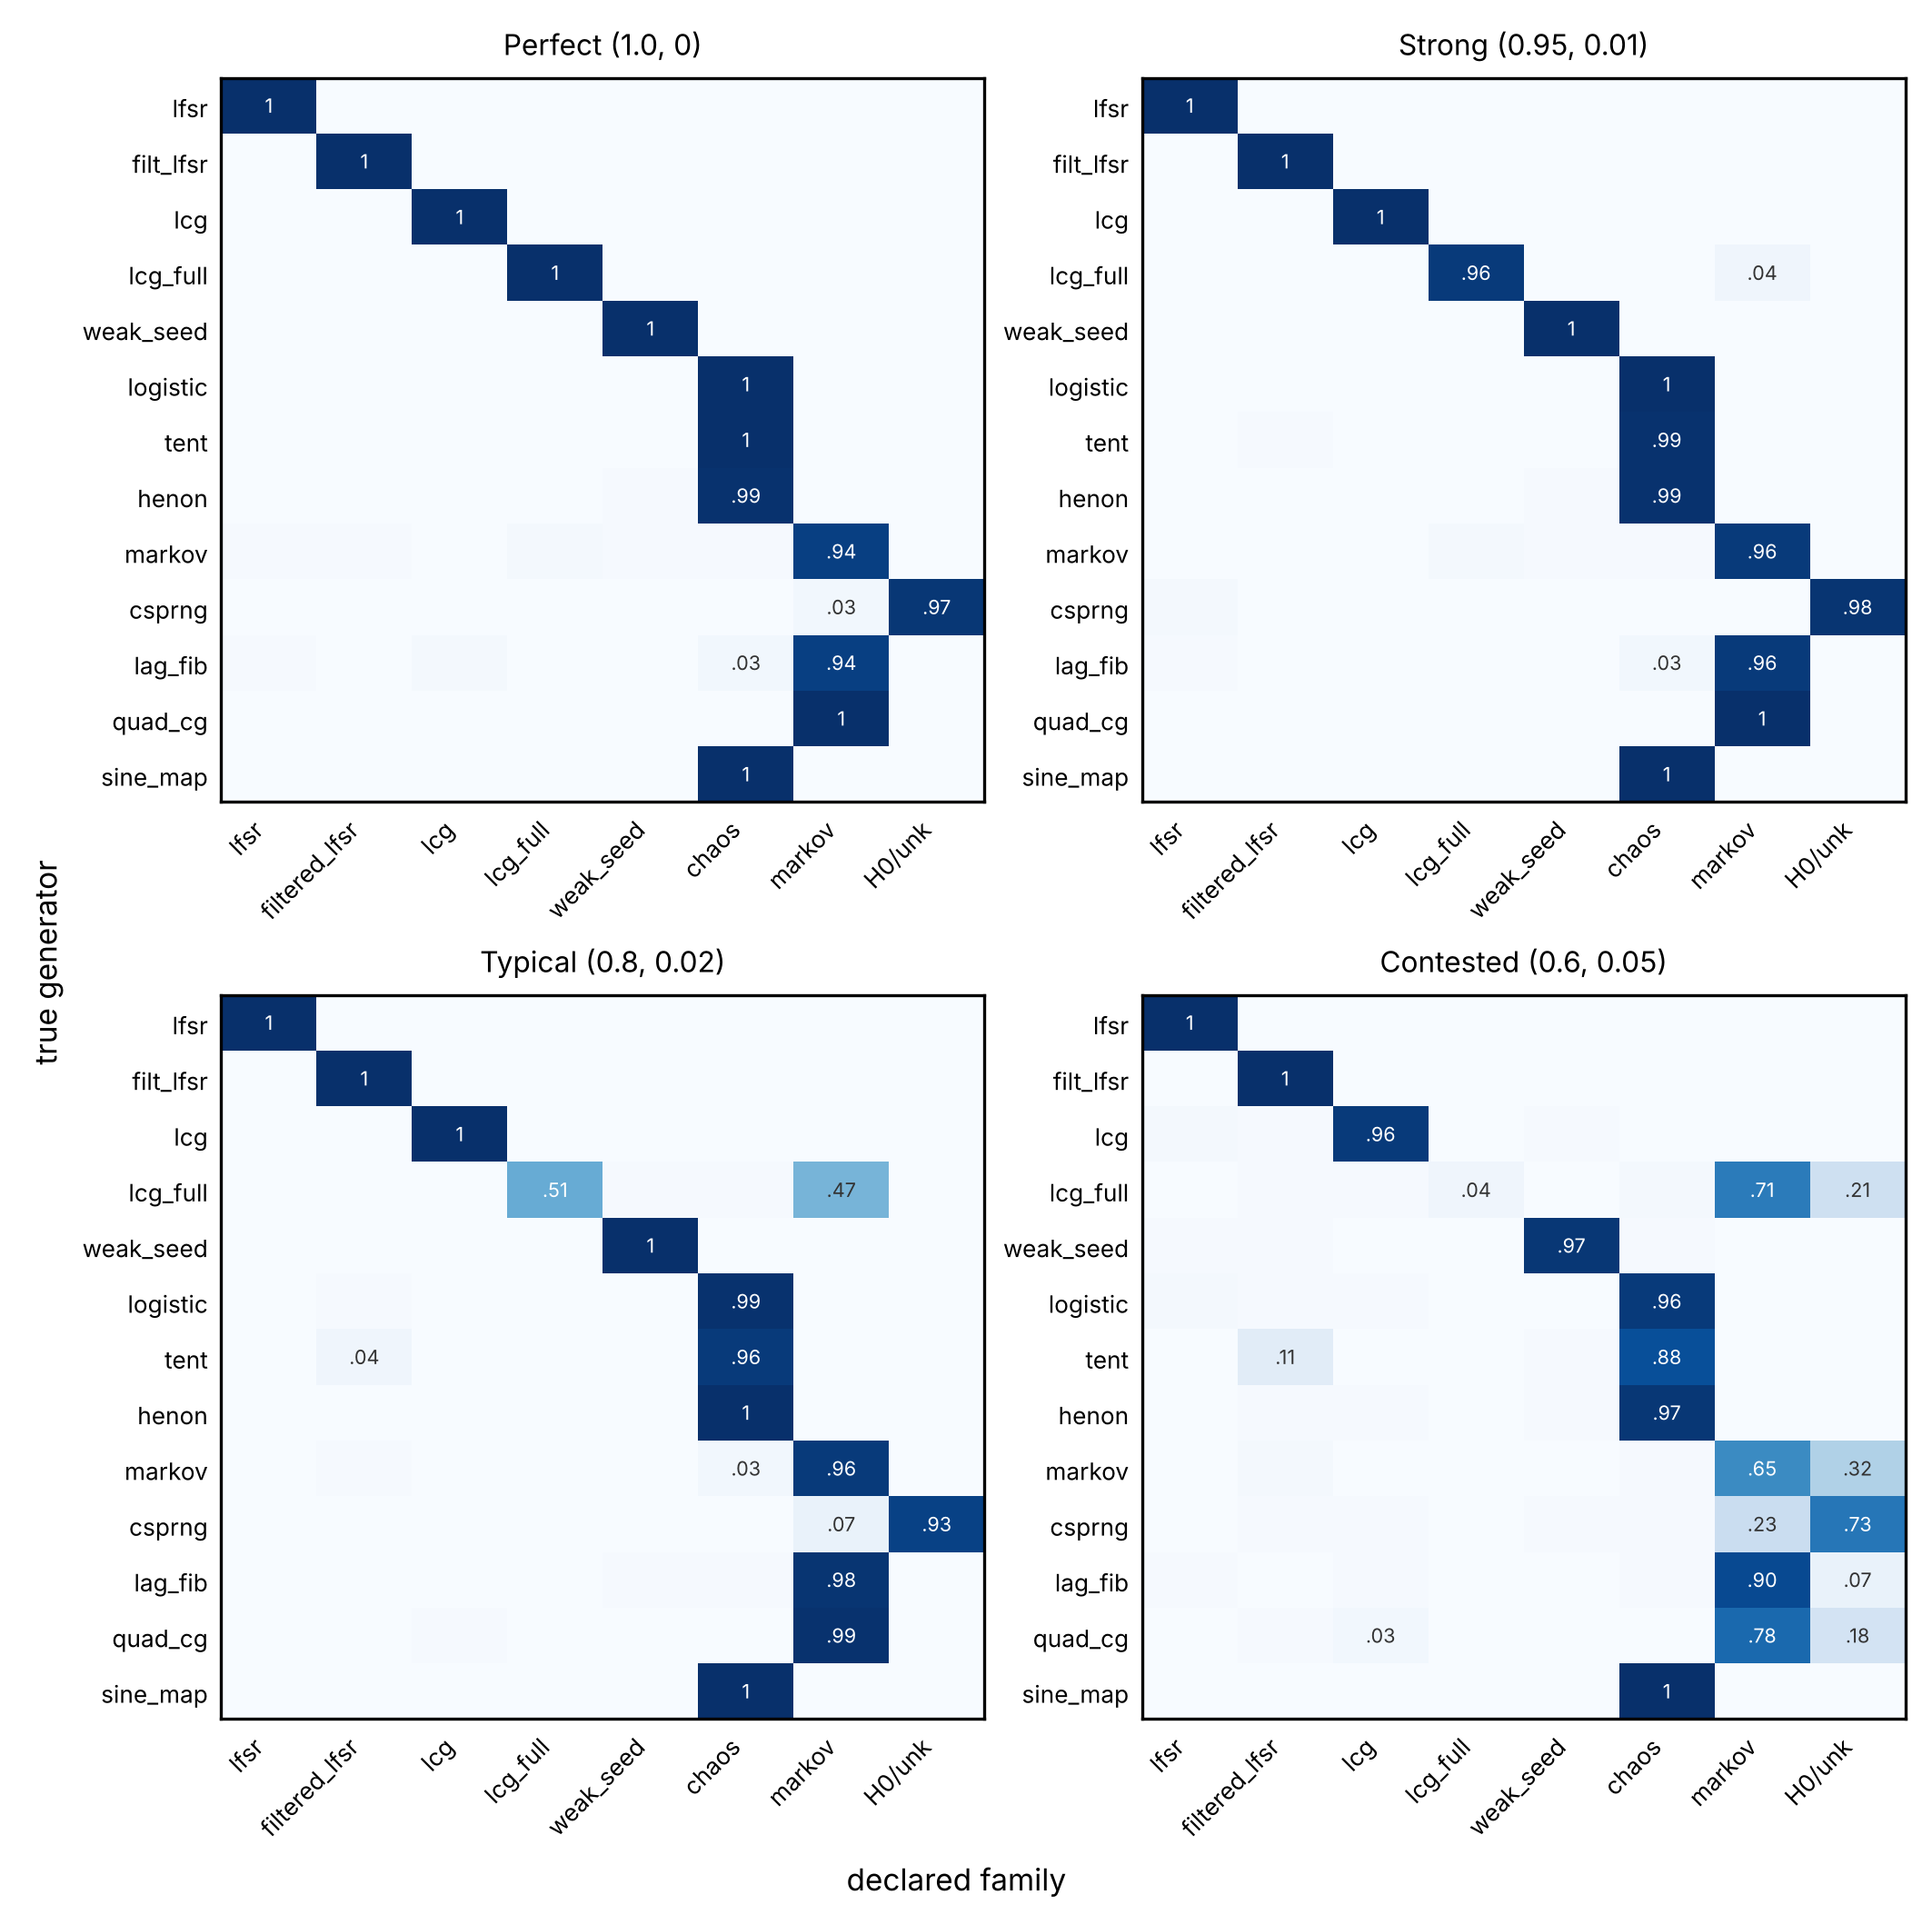
\includegraphics[width=0.45\textwidth]{fig_confusion.png}
\caption{Family confusion matrices (true generator vs declared family), one per
sensor, $100$ seeds per cell. Rows are the thirteen generators including the
three held-out families and the CSPRNG; columns are the declared families and
$H_0$/unknown. The diagonal stays clean for identifiable families; held-out and
unbreakable sources degrade to Markov/$H_0$, never to a false algebraic claim,
even on the contested sensor.}
\label{fig:confusion}
\end{figure}

\begin{table}[t]
\centering
\caption{Identification accuracy / hard false-ID across sensors (100 seeds).}
\label{tab:ident}
\setlength{\tabcolsep}{3.4pt}
\footnotesize
\begin{tabular}{@{}lcccc@{}}
\toprule
 & Perfect & Strong & Typical & Contested \\
Generator & \multicolumn{4}{c}{accuracy / hard false-ID} \\
\midrule
LFSR         & 1.00 / .00 & 1.00 / .00 & 1.00 / .00 & 1.00 / .00 \\
filt.\ LFSR  & 1.00 / .00 & 1.00 / .00 & 1.00 / .00 & 1.00 / .00 \\
LCG          & 1.00 / .00 & 1.00 / .00 & 1.00 / .00 & 0.96 / .04 \\
weak-seed    & 1.00 / .00 & 1.00 / .00 & 1.00 / .00 & 0.97 / .00 \\
chaos (log.) & 1.00 / .00 & 1.00 / .00 & 0.99 / .00 & 0.96 / .00 \\
Markov       & 0.94 / .05 & 0.96 / .01 & 0.96 / .01 & 0.65 / .02 \\
CSPRNG       & 0.97 / .00 & 0.98 / .00 & 0.93 / .00 & 0.73 / .03 \\
\bottomrule
\end{tabular}
\end{table}

\begin{table}[t]
\centering
\caption{Identification against conventional identifiers on identical episodes
($100$ seeds $\times$ $10$ generators per sensor). Acc.: in-bank accuracy;
Unk.: CSPRNG reported unknown; hard false-ID over all episodes / over
out-of-bank episodes; mean hops to a correct declaration.}
\label{tab:idbase}
\setlength{\tabcolsep}{3.2pt}
\footnotesize
\begin{tabular}{@{}llcccc@{}}
\toprule
Sensor & Method & Acc. & Unk. & Hard false-ID & Hops \\
\midrule
Typical   & bank $+H_0$ (ours) & \textbf{0.99} & \textbf{0.89} & \textbf{.004} / \textbf{.005} & 18.8 \\
          & pairwise SPRT      & 0.98 & 0.00 & .103 / .235 & 16.9 \\
          & fixed-length LRT   & 0.94 & 0.00 & .128 / .230 & 30 \\
          & learned classifier & 0.61 & 0.24 & .318 / .482 & 140 \\
\midrule
Contested & bank $+H_0$ (ours) & \textbf{0.93} & \textbf{0.82} & \textbf{.009} / \textbf{.018} & 14.5 \\
          & pairwise SPRT      & 0.91 & 0.00 & .154 / .268 & 12.4 \\
          & fixed-length LRT   & 0.90 & 0.00 & .222 / .417 & 30 \\
          & learned classifier & 0.47 & 0.26 & .303 / .412 & 140 \\
\bottomrule
\end{tabular}
\end{table}

\subsection{The value of the sensor-aware likelihood}
We replace \eqref{eq:emit} with a naive clean-match score to see what the
sensor model is worth. While detections are plentiful the two scores agree. As
$P_d$ falls to $0.5$ (at $P_{fa}=0.05$), the naive bank drops to $0.60$
accuracy against $0.98$ and needs $21.1$ hops against $15.3$. The reason is
that it reads a missed hop as evidence against the truth and a phantom as
evidence for a wrong generator. For a single recovery algorithm the effect is a
cliff. Plain Berlekamp--Massey recovers an $L{=}7$ LFSR on every run at
$P_d{=}1$ and on \emph{no} run for any $P_d<1$, while the state-enumeration
recovery under \eqref{eq:emit} holds $1.00$ across the whole sweep. That gap is
what modelling the sensor inside the likelihood buys.

\subsection{Mis-specified sensor}
The bank scores with the same $(P_d,P_{fa})$ that generated the data. In the
field the assumed values will differ from the true ones, so
Fig.~\ref{fig:mismatch} sweeps the assumed value against the true one.
Identification is robust to an over-optimistic $P_d$. Accuracy stays high
across the off-diagonal, because a missed hop only leaves out a likelihood
factor and does not corrupt one. The hard false-ID rate under a mis-specified
$P_{fa}$ also stays low. The system therefore does not need an exact sensor
model: when its sensor estimate is wrong, performance degrades gently.

\begin{figure}[t]
\centering
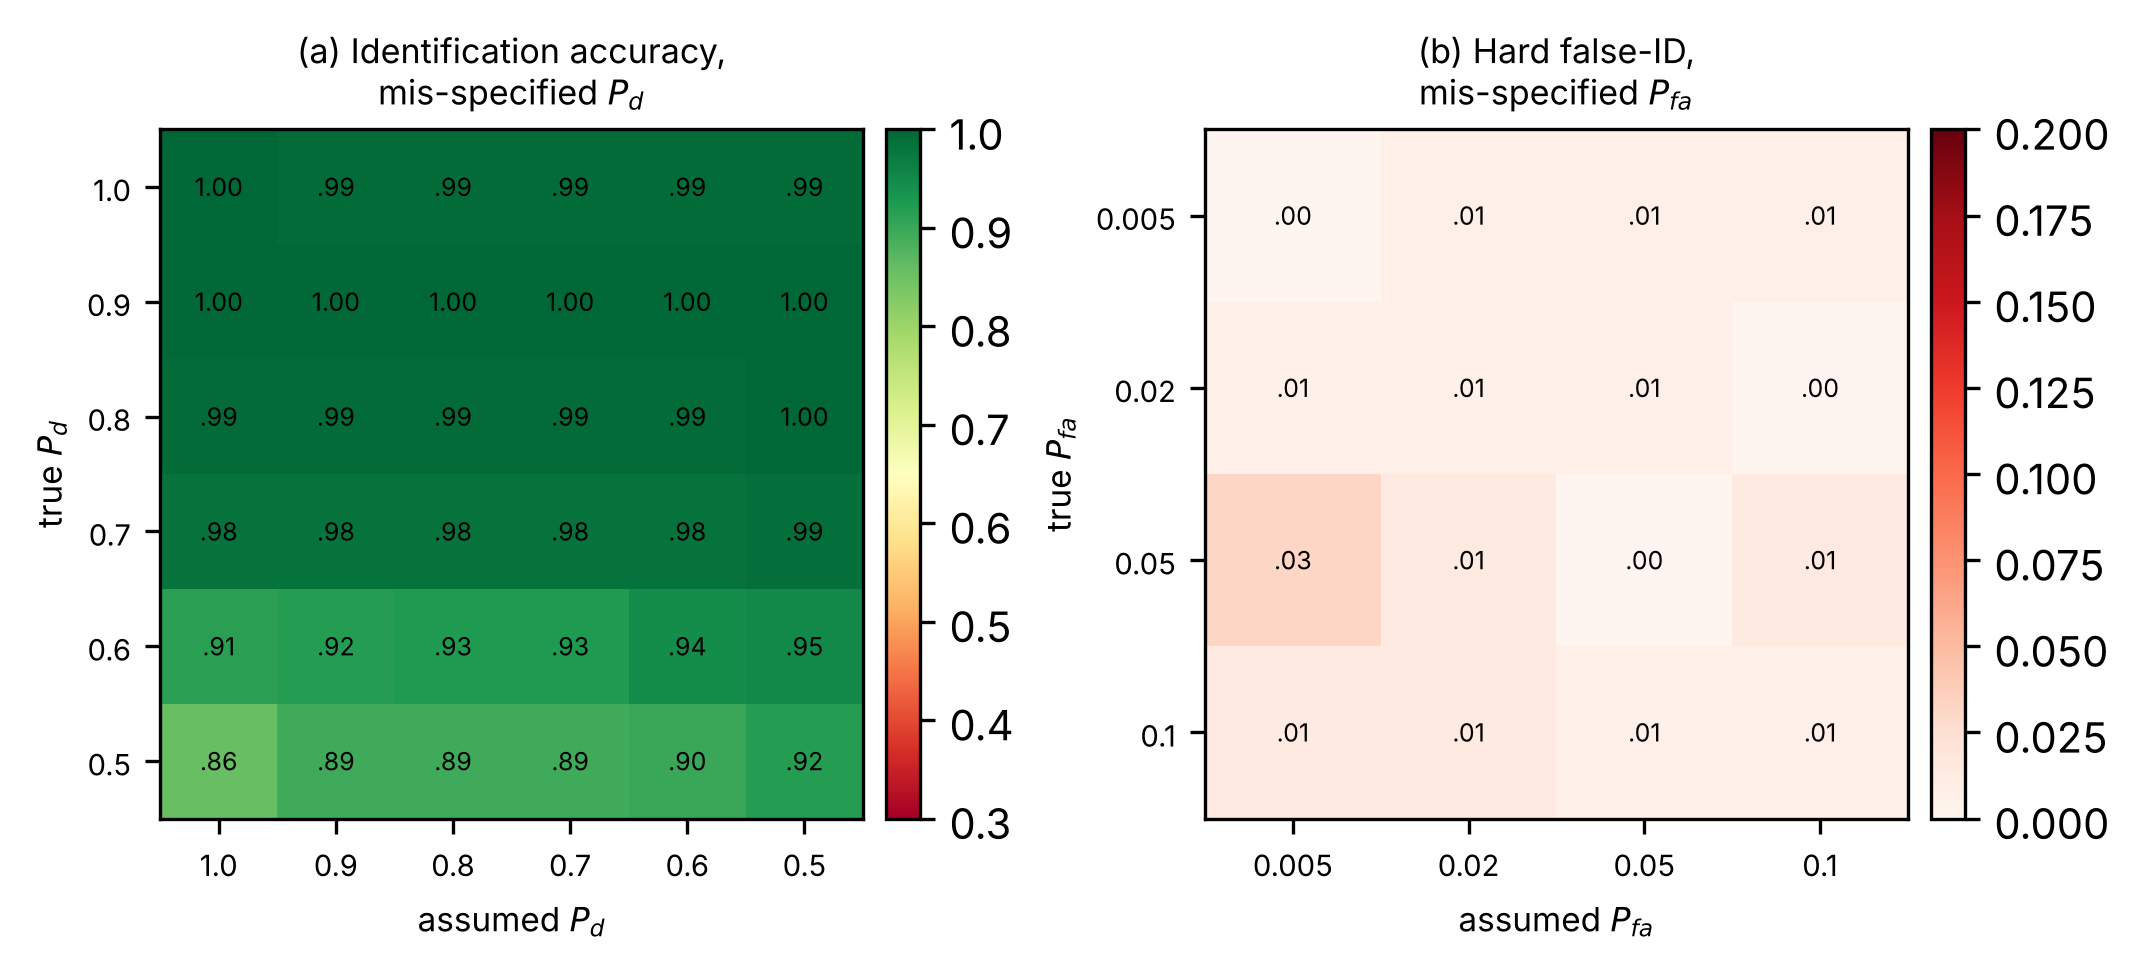
\includegraphics[width=\columnwidth]{fig_mismatch.png}
\caption{Mis-specified sensor. (a) Identification accuracy as the assumed $P_d$
(columns) departs from the true $P_d$ (rows). (b) Hard false-ID as the assumed
$P_{fa}$ departs from the true $P_{fa}$. Accuracy and safety hold across a wide
mismatch band.}
\label{fig:mismatch}
\end{figure}

\subsection{Next-channel prediction and conformal sets}
Fig.~\ref{fig:results} collects the headline prediction results. Panel~(b)
carries the central claim. On the held-out lagged-Fibonacci generator the
proposed predictor reaches $1.00$ steady-state top-1, while an
identification-only bank manages $0.38$. The universal context-mixing expert
recovers the order-2 rule, which no bank expert can represent. On a keyed
CSPRNG both correctly fall to chance. Table~\ref{tab:predict} gives the numbers
at each operating point; the advantage holds on the typical and contested
sensors.

\emph{Against external predictors.} Table~\ref{tab:predbase} runs three
predictors that owe nothing to the bank on the episodes of
Table~\ref{tab:predict}. The trained LSTM is the instructive case. It matches
the bank on the LFSR it was trained on ($1.00$, falling to $0.54$ on the
contested sensor where the bank holds $1.00$). On the held-out lagged-Fibonacci
and quadratic generators, however, it scores $0.01$--$0.13$, at or below
chance. It has learned its training families and has not learned how to pick up
a new rule in-context. PPM-C is training-free and partly recovers the
lagged-Fibonacci rule on the strong sensor ($0.74$), but it has no sensor
model. Every missed or ambiguous slot breaks its context, so it falls to $0.42$
and $0.21$ as the sensor degrades, and it never predicts the LFSR well. On the
sine map no predictor beats a statistical learner, and PPM-C ties the mixture
on the strong sensor.

Panel~(c) shows the conformal set tracking the target coverage diagonal while
a fixed top-3 shortlist sits well below it. A fixed shortlist covers only
$0.51$ on a Markov hopper and $0.19$ on a CSPRNG. The conformal set holds
$\geq 0.90$ by growing its size, from one tone on a pinned-down LFSR up to the
whole plan on the CSPRNG. The data therefore sets the number of transmit
frequencies.

\begin{figure*}[b]
\centering
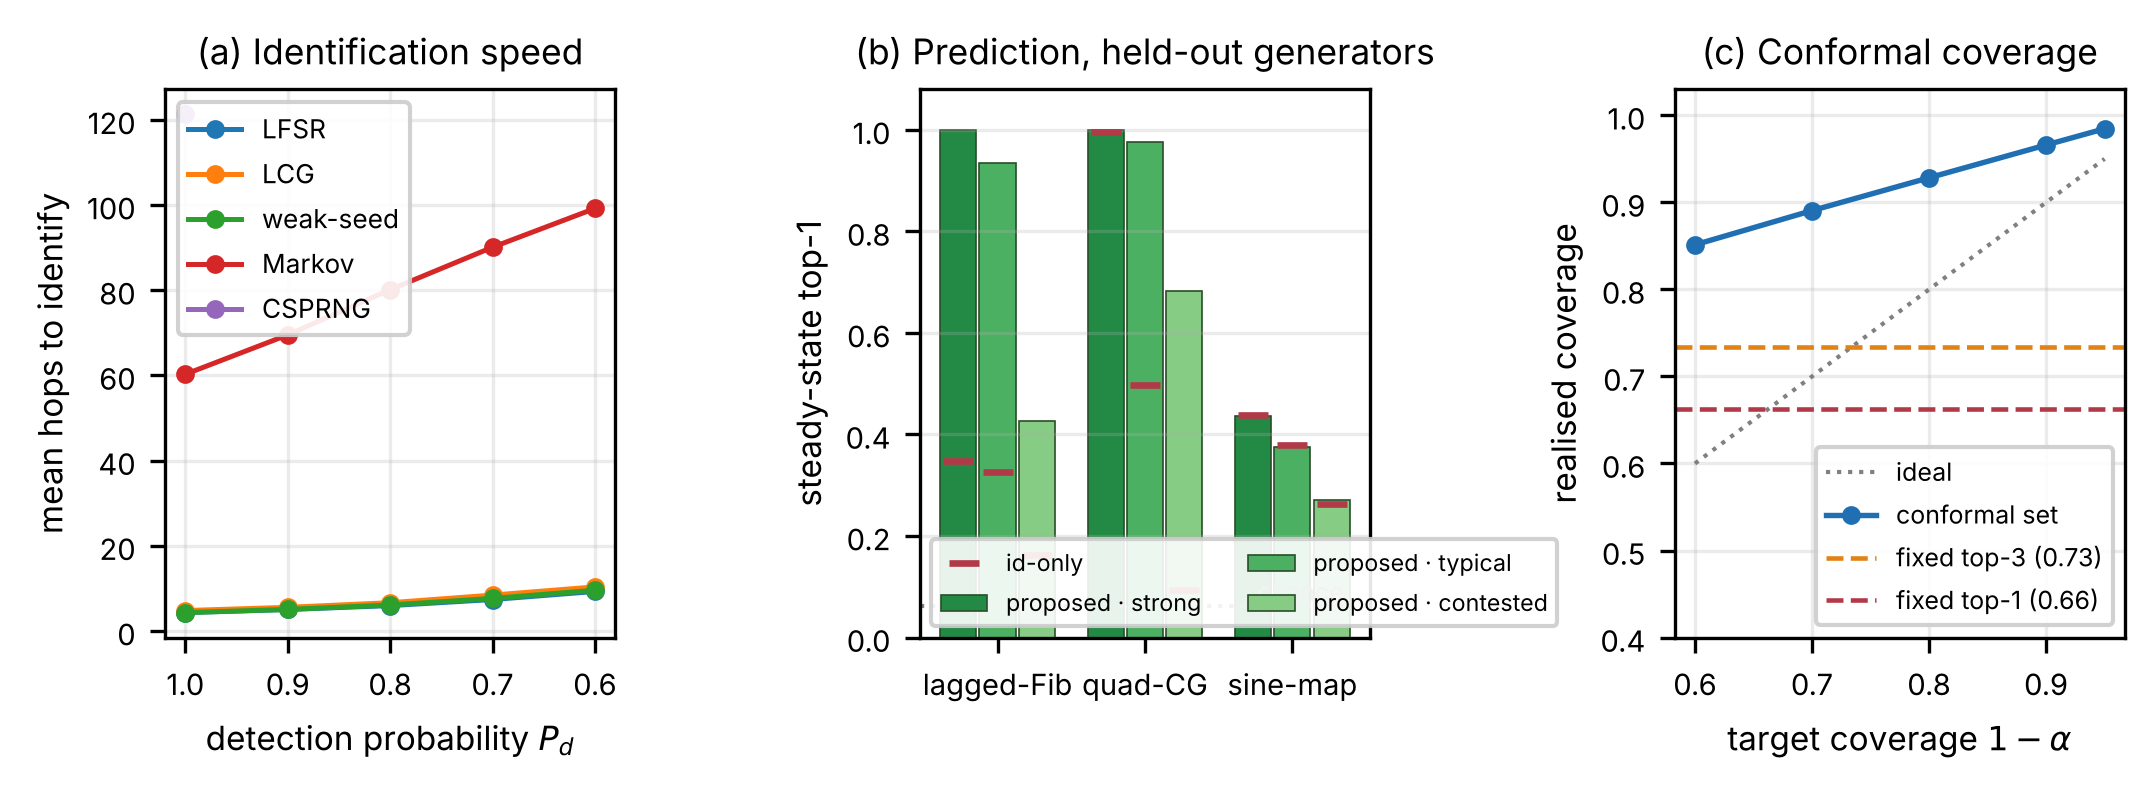
\includegraphics[width=0.8\textwidth]{fig_results.png}
\caption{(a) Mean hops-to-identify vs $P_d$: deterministic families need a
handful of hops, Markov an order of magnitude more. (b) Steady-state top-1
next-channel accuracy on the three held-out generators (bars: proposed, across
sensors; red ticks: identification-only bank); the dotted line is chance. (c)
Conformal coverage calibration: the set tracks the target, fixed shortlists do
not.}
\label{fig:results}
\end{figure*}

\begin{table}[t]
\centering
\caption{Steady-state top-1 next-channel accuracy, proposed predictor (P) vs
identification-only bank (I), across sensors (chance $=0.0625$, 30 seeds).}
\label{tab:predict}
\setlength{\tabcolsep}{3pt}
\footnotesize
\begin{tabular}{@{}lcccccc@{}}
\toprule
 & \multicolumn{2}{c}{Strong} & \multicolumn{2}{c}{Typical} & \multicolumn{2}{c}{Contested} \\
Generator & P & I & P & I & P & I \\
\midrule
LFSR (in-bank)          & 1.00 & 1.00 & 1.00 & 1.00 & 1.00 & 1.00 \\
lagged-Fib.\ (held out) & \textbf{1.00} & 0.38 & \textbf{0.94} & 0.33 & \textbf{0.43} & 0.16 \\
quad.-CG (held out)     & \textbf{1.00} & 0.90 & \textbf{0.98} & 0.50 & \textbf{0.68} & 0.09 \\
sine map (held out)     & 0.43 & 0.43 & 0.38 & 0.38 & 0.27 & 0.26 \\
CSPRNG (control)        & 0.07 & 0.07 & 0.07 & 0.06 & 0.06 & 0.06 \\
\bottomrule
\end{tabular}
\end{table}

\begin{table}[t]
\centering
\caption{External predictors on the episodes of Table~\ref{tab:predict}:
online first-order Markov (M1), online PPM-C (PPM) and an LSTM trained on the
in-bank families. Steady-state top-1; compare column P of
Table~\ref{tab:predict}.}
\label{tab:predbase}
\setlength{\tabcolsep}{2.4pt}
\footnotesize
\begin{tabular}{@{}lccccccccc@{}}
\toprule
 & \multicolumn{3}{c}{Strong} & \multicolumn{3}{c}{Typical} & \multicolumn{3}{c}{Contested} \\
Generator & M1 & PPM & LSTM & M1 & PPM & LSTM & M1 & PPM & LSTM \\
\midrule
LFSR        & 0.34 & 0.43 & 1.00 & 0.25 & 0.26 & 1.00 & 0.11 & 0.11 & 0.54 \\
lagged-Fib. & 0.37 & 0.74 & 0.09 & 0.27 & 0.42 & 0.13 & 0.12 & 0.21 & 0.07 \\
quad.-CG    & 0.83 & 0.82 & 0.04 & 0.52 & 0.49 & 0.01 & 0.10 & 0.10 & 0.06 \\
sine map    & 0.40 & 0.44 & 0.38 & 0.24 & 0.28 & 0.36 & 0.10 & 0.14 & 0.28 \\
CSPRNG      & 0.07 & 0.06 & 0.08 & 0.07 & 0.06 & 0.07 & 0.06 & 0.04 & 0.07 \\
\bottomrule
\end{tabular}
\end{table}

\subsection{Multi-tone response: hops denied}
Fig.~\ref{fig:denial} measures the end quantity directly. A tone is funded on
the $\min(|S_t|,B)$ most probable channels of the conformal set (target
$0.9$). A hop counts as denied when its true channel is funded, and we score
every slot, including the ones that are not clean. With the budget
unconstrained the denied fraction is $0.90$--$1.00$ for every generator on all
three sensors, so the guarantee transfers. What differs between generators is
the price. On the typical sensor an LFSR or LCG is denied at $1.00$ with one
tone (the set asks for $1.2$). The held-out lagged-Fibonacci and sine map need
$2.4$ and $5.6$ tones. The Markov hopper and CSPRNG need $14$ of $16$ channels,
which is the system reporting that only barrage works. A fixed top-3 shortlist
denies every LFSR hop but only $0.35$ of Markov hops and $0.18$ of CSPRNG hops.
The price rises as the sensor degrades: on the contested sensor the
lagged-Fibonacci set grows to $9.7$ tones, and four tones deny only $0.64$ of
its hops.

\begin{figure}[t]
\centering
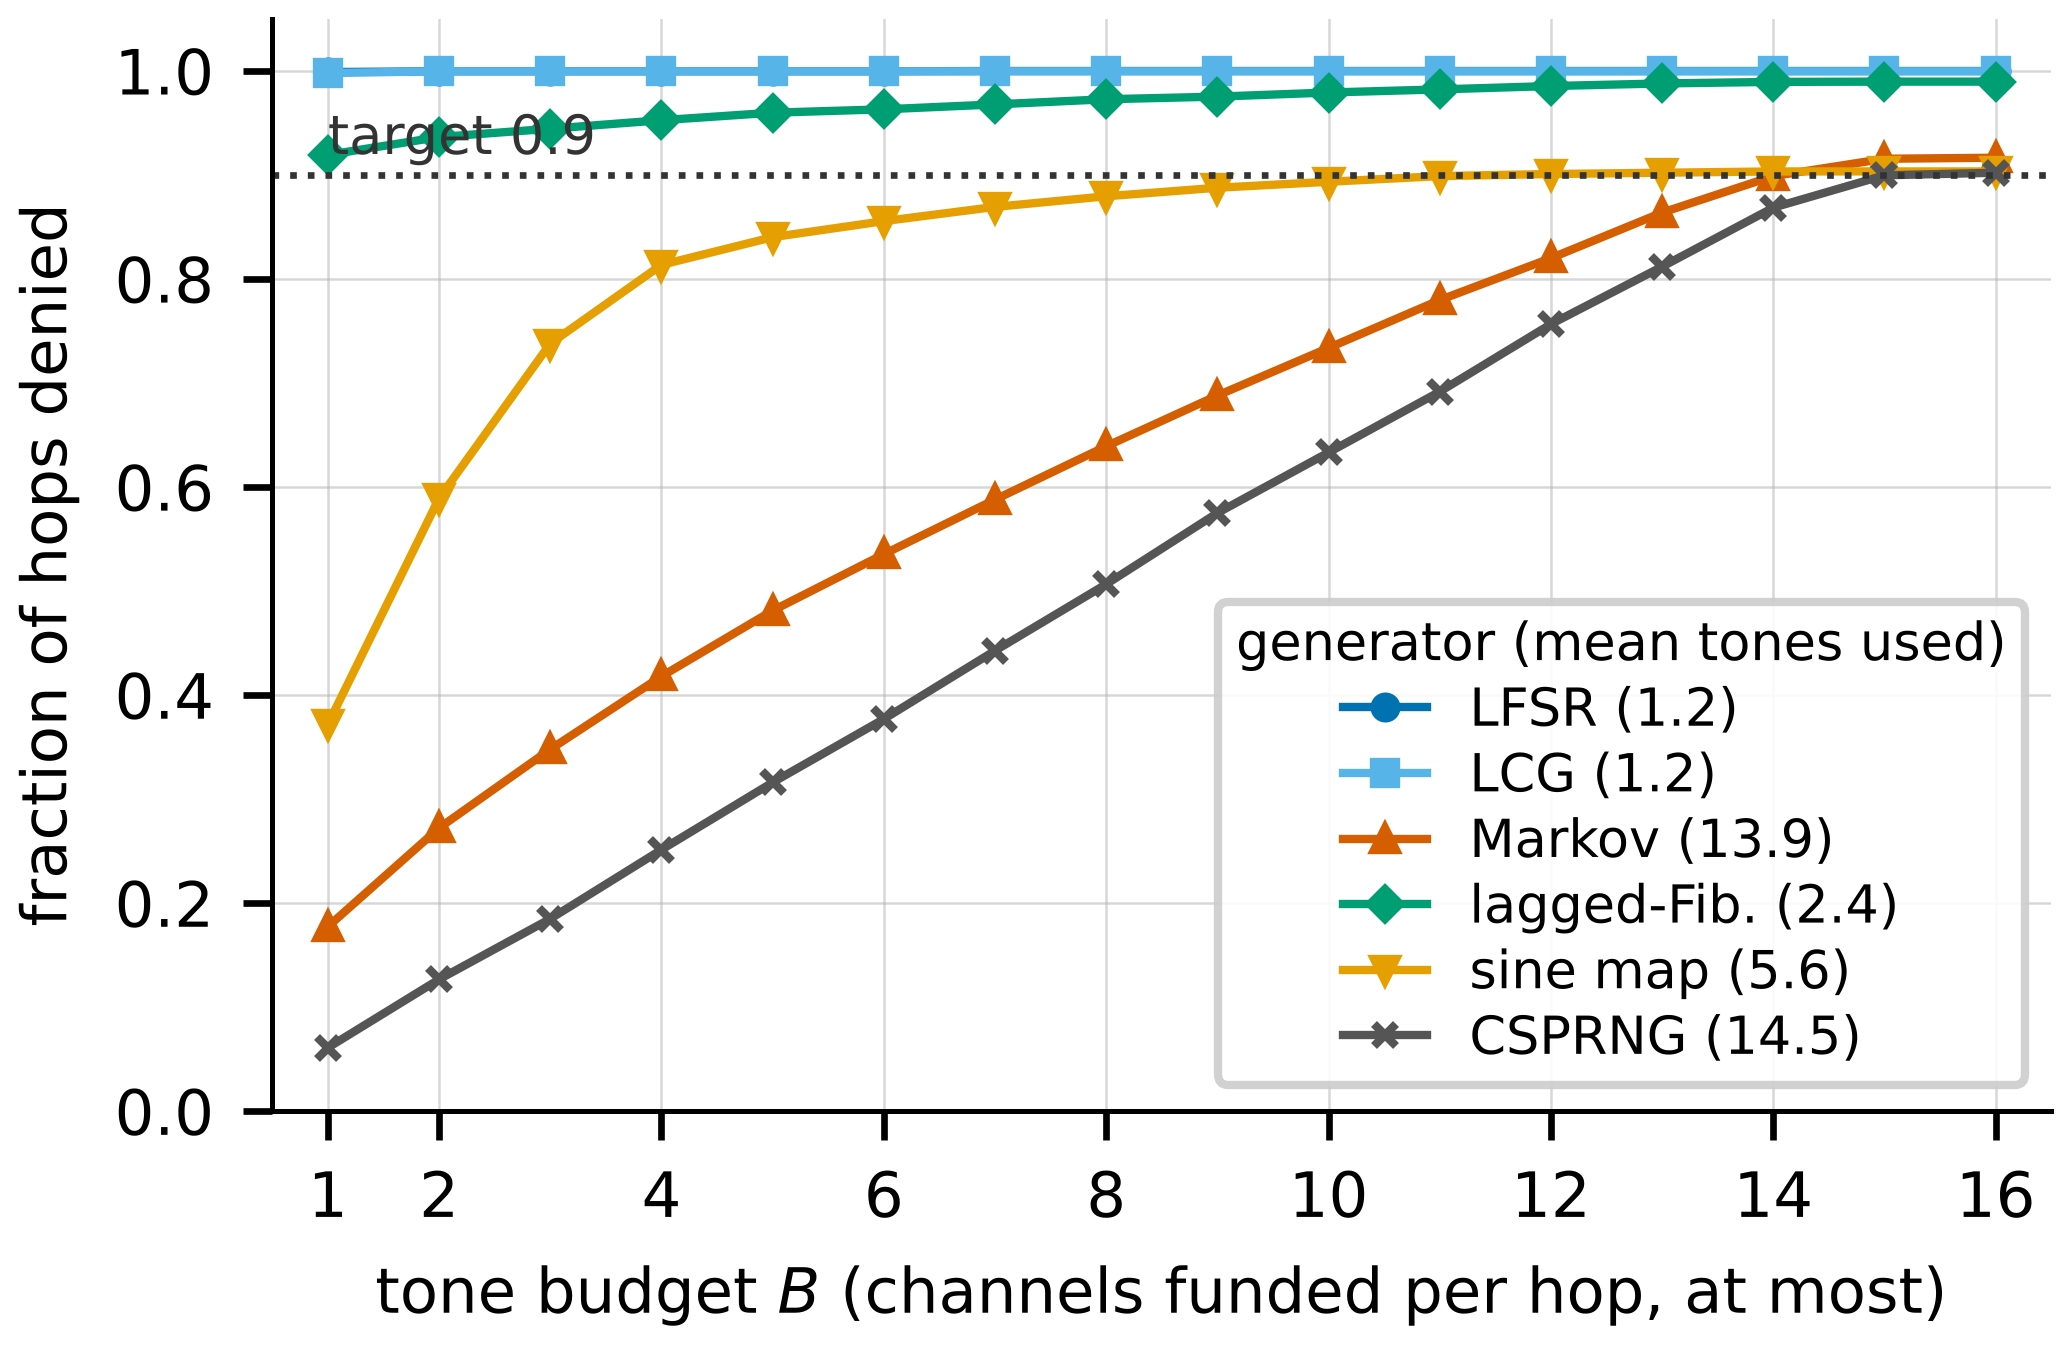
\includegraphics[width=0.78\columnwidth]{fig_denial.png}
\caption{Fraction of hops denied against the tone budget $B$ on the typical
sensor (conformal target $0.9$, $30$ seeds, $140$ hops). Legend: mean tones
the set asks for when $B$ is unconstrained.}
\label{fig:denial}
\end{figure}

\subsection{Per-slot compute time}
We time the unoptimised NumPy implementation on one core of a $2.1$\,GHz Xeon.
At $M{=}16$ the median time per slot is $0.79$\,ms in the identification bank
(seven experts and $H_0$), $1.86$\,ms in the predictor (bank, universal and
rule-search experts) and $0.06$\,ms on the conformal set and tone selection.
At $M{=}64$ the figures are $0.87$, $2.29$ and $0.07$\,ms. Building the
experts' tables is a one-off cost of $0.5$\,s. The total of about $3$\,ms fits
the dwell of a hopper running at a few hundred hops per second. It grows little
with $M$ because the cost follows the number of candidate parameterisations,
not the number of channels. Two costs are larger. The predictor's search
experts fire in bursts (95th percentile $17$\,ms), and the switch tracker,
which carries several anchored banks, takes $46$\,ms ($82$\,ms at $M{=}64$).

\subsection{Switch tracking and the cost of identification}
Table~\ref{tab:switch} replays $24$ random switch plans over all thirteen
algorithms ($113$ switches) through the switch tracker. It detects
$95$--$97\%$ of switches, with a median delay of $0$ hops on a perfect sensor
and $12$ on a contested one. Dangerous locks stay at or below $0.015$ per
regime (two across the whole contested run). Finally, we compare the measured
hops-to-identify with the information-theoretic lower bound
$\mathbb{E}[\tau]\geq\log((1-\delta)/\delta)/D$, where the posterior log-odds
drift $D$ is estimated on the runs. The measured value sits within
$1.3$--$2.7\times$ the bound (mean efficiency $2.2\times$, always at or above
the floor). The stopping rule is therefore close to the fastest that any
identifier could achieve on these streams.

\begin{table}[t]
\centering
\caption{Switch tracking: 24 random plans over 13 algorithms (113 switches),
$M=16$.}
\label{tab:switch}
\setlength{\tabcolsep}{3pt}
\footnotesize
\begin{tabular}{@{}lcccc@{}}
\toprule
Sensor & Perfect & Strong & Typical & Contested \\
\midrule
Switches detected        & 97\% & 97\% & 97\% & 95\% \\
Delay, median/90th (hops)& 0/6  & 1/7  & 4/12 & 12/34 \\
Dangerous locks /regime  & .000 & .000 & .000 & .015 \\
Top-1, hops 6--10        & 0.72 & 0.65 & 0.53 & 0.20 \\
\bottomrule
\end{tabular}
\end{table}

\subsection{Operator dashboard: the Control room}
\label{sec:dashboard}
To show the loop to an operator, and to let a person try to defeat it, we built
a browser dashboard on top of the same implementation. Its \emph{Control room}
page (Fig.~\ref{fig:control}) is a live engagement. A local server runs the
switch tracker of Sec.~\ref{sec:switch} one slot per request. The operator
drives the transmitter, and the system sees only the sensor's detections. The
operator chooses the channel count ($4$--$64$), the window ($20$--$1000$ hops)
and the sensor (Perfect, the three presets of Sec.~\ref{sec:setup}, or a custom
$(P_d,P_{fa})$). Pressing one of the thirteen algorithm buttons puts the radio
on air with that generator. Pressing another switches it mid-engagement, and
every switch draws a fresh secret from the same reconnaissance ranges as the
experiments, so the system never gets a warm start. Information parity holds
here too. The true algorithm, its secret and the true channel are drawn only
as overlays for the audience, after the slot has been scored.

The page has four panels. The \emph{hop chart} plots the sensor detections and,
one slot ahead, the conformal set the system commits to for the next hop: a
ring on the top channel, plus extra tones when the top channel is under $90\%$.
A band above the chart shows the family the system believes is on air, and a
band below shows what the transmitter actually runs. \emph{The system's view}
gives the lock state, the declared family and its posterior, the estimated
switch slot, the recovered secret next to the true one, the next-channel call,
and the family race, including $H_0$ and the switch posterior. A
\emph{whole-session} strip plots truth against belief with the rolling top-1
rate and marks every operator switch and every detection. An event log and a
per-algorithm table score each regime by switch delay, final answer, hops to
lock and hit rate. A ``max transmit frequencies'' control caps the tone budget
$B$ of the response.

Fig.~\ref{fig:control} is a $202$-hop session on the typical sensor at $M{=}16$.
The radio runs an LFSR, then a weak-seed PRNG from hop $73$, then the held-out
lagged-Fibonacci generator from hop $142$. The LFSR locks after $6$ hops. Both
switches are flagged $2$ hops after they happen and dated to the exact slot.
The weak-seed PRNG locks $9$ hops after its switch. The lagged-Fibonacci
generator has no expert, and the bank does not force an algebraic match. It
labels the generator with its nearest statistical description (Markov, $96\%$),
while the universal and rule-search experts carry the forecast. Over the
session the next-hop set caught $191$ of $201$ hops ($95\%$, $1.2$ tones on
average; exact top-1 $94\%$), against $8\%$ for a random set of the same size.
In the regime after the last switch it caught $54$ of $61$. The page works as a
demonstration, and it also works as an informal red-team test: the operator can
switch at any slot, try unseen generators, and watch whether a confident false
claim ever appears.

\begin{figure*}[t]
\centering
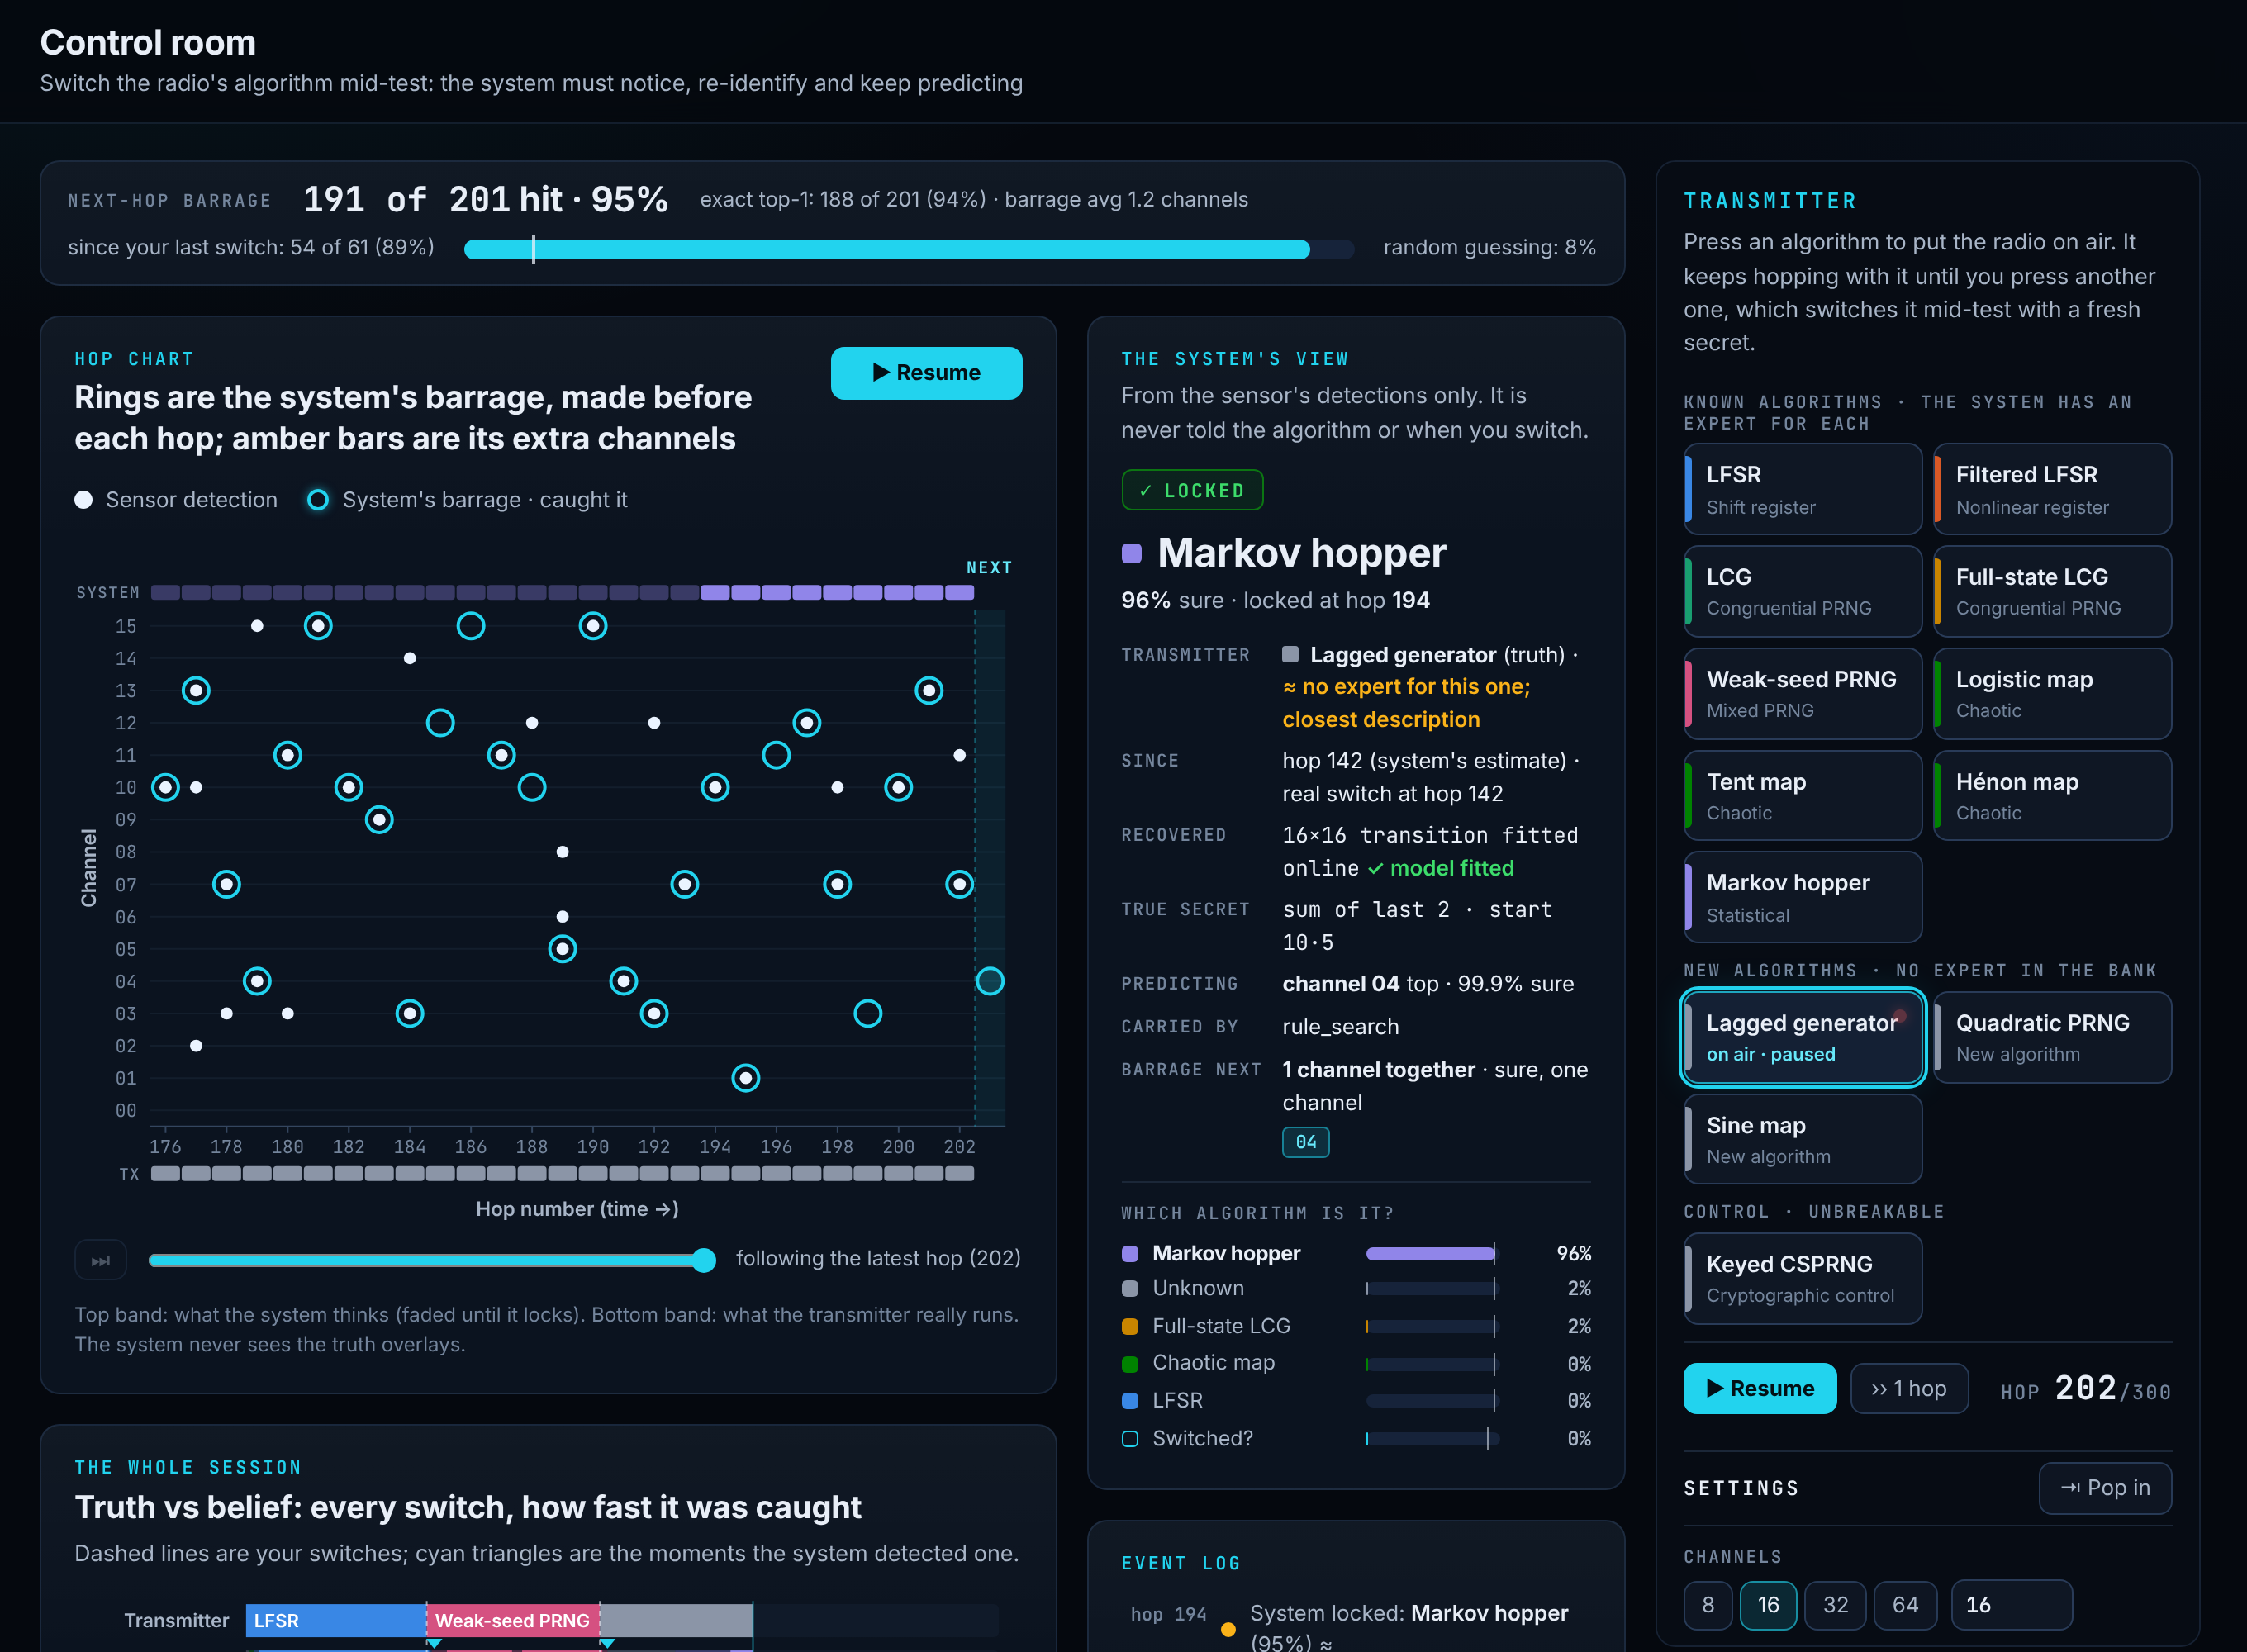
\includegraphics[width=0.92\textwidth]{fig_control_room.png}
\caption{The Control room dashboard, paused at hop $202$ of a live session
(typical sensor $P_d{=}0.8$, $P_{fa}{=}0.02$, $M{=}16$). The operator has
switched the transmitter (right) from LFSR to weak-seed PRNG to the held-out
lagged-Fibonacci generator. Hop chart: white dots are sensor detections, cyan
rings are the system's next-hop set committed before each hop; the top band is
the system's belief and the bottom band (TX) is the truth. The system's view
shows the lock, the family race with $H_0$ and the switch posterior, and the
next-channel call. Top bar: $191/201$ next hops caught at $1.2$ tones on
average.}
\label{fig:control}
\end{figure*}

%=======================================================================
\section{Discussion}
\label{sec:discussion}
%=======================================================================
Every deterministic family is scored by enumerating its parameters through
\eqref{eq:emit}. This single design choice explains three results:
identification in single-digit hops, a cost that scales as $1/P_d$, and
immunity to false alarms, because a phantom scales every candidate equally and
cancels.

The dangerous error is a confident, false claim of an algebraic break, which
would send an operator after the wrong generator. That rate is at most $0.05$
across every sensor and all coverage episodes. A closed-set test without $H_0$
makes the same error on $0.24$ of out-of-bank episodes. In-bank accuracy is
almost the same with or without $H_0$, so the reason to include an explicit
generative $H_0$ is this gap in safety.

Any bank is finite, and an adversary can pick a generator outside it. Because
the Fixed-Share mixture weights experts by recent skill, the training-free
universal expert takes over within a few slots. The lagged-Fibonacci result
($1.00$ vs $0.38$) is the clearest case. Where a source has only statistical
structure (sine map, Markov), the mixture does no better than its best
statistical learner, and we do not expect any predictor to.

All results are simulated with a slot-synchronous, i.i.d.\ sensor; hop-timing
jitter, bursty fades and interleaved emitters are future work. $M=16$ confounds
the full-state LCG (period $\leq 16$) with a Markov cycle. The generators and
experts share authors, which the held-out families mitigate but do not remove.
The e-process guarantee is proven only for in-bank truths; out-of-bank
protection is empirical, via $H_0$. The learned baselines are our own, trained
on our simulator, and are not re-implementations of published models. Timings
are for unoptimised single-core Python.

%=======================================================================
\section{Conclusion}
%=======================================================================
FHBP takes the imperfect detections of a passive sensor and turns them into a
single likelihood score per slot. That one score is used in four ways: to test
the stream against a bank of known generators, to predict the next channel
without any training, to track when the emitter switches its algorithm, and to
build a prediction set with a statistical guarantee. With it the system
identifies known generators within a few hops while keeping false algebraic
claims at or below $0.05$, keeps predicting on generators it was never designed
for, and notices when the opponent changes algorithm in the middle of an
engagement. Its coverage guarantee does not depend on any assumed data
distribution, and the guarantee carries over to the multi-tone response.

The individual building blocks come from established theory. What is new is
joining them through one sensor-aware likelihood and applying the result to
frequency hopping; to our knowledge, no earlier system identifies the
generator, predicts the next hop, tracks a switch and calibrates a response
from the same lossy passive stream. Future work will test the system with
bursty, non-ideal sensors and real recorded data, extend it to larger channel
sets, compare it against published learned predictors retrained on our data,
and develop a faster method for tracking switches.


%=======================================================================
\begin{thebibliography}{00}
\bibitem{li2020lstm} G. Li \emph{et al.}, ``LSTM-based frequency hopping
sequence prediction,'' in \emph{Proc. WCSP}, 2020.
\bibitem{li2021china} G. Li \emph{et al.}, ``Frequency-hopping frequency
reconnaissance and prediction for non-cooperative communication network,''
\emph{China Commun.}, 2021.
\bibitem{zhu2023recovery} J. Zhu \emph{et al.}, ``Deep-learning-based recovery
of frequency-hopping sequences for anti-jamming applications,''
\emph{Electronics}, vol.~12, no.~3, 2023.
\bibitem{basak2024spectrum} S. Basak \emph{et al.}, ``Spectrum prediction for
protocol-aware RF jamming,'' \emph{IEEE Trans. Cogn. Commun. Netw.}, 2024.
\bibitem{strickland2023} C. Strickland \emph{et al.}, ``Predicting jamming
systems frequency hopping sequences using artificial neural networks,'' in
\emph{Proc. IEEE SoutheastCon}, 2023.
\bibitem{tao2025transformers} T. Tao, A. Doshi, V. Kalra, M. He, and
M. Barkeshli, ``(How) can transformers predict pseudo-random numbers?'' in
\emph{Proc. ICML}, 2025.
\bibitem{lee2020detection} K.-G. Lee \emph{et al.}, ``Detection of
frequency-hopping signals with deep learning,'' \emph{IEEE Commun. Lett.}, 2020.
\bibitem{baum1994} C. W. Baum and V. V. Veeravalli, ``A sequential procedure for
multihypothesis testing,'' \emph{IEEE Trans. Inf. Theory}, 1994.
\bibitem{dragalin1999} V. P. Dragalin, A. G. Tartakovsky, and V. V. Veeravalli,
``Multihypothesis sequential probability ratio tests,'' \emph{IEEE Trans. Inf.
Theory}, 1999.
\bibitem{ramdas2023} A. Ramdas \emph{et al.}, ``Game-theoretic statistics and
safe anytime-valid inference,'' \emph{Statist. Sci.}, vol.~38, no.~4, 2023.
\bibitem{gutman1989} M. Gutman, ``Asymptotically optimal classification for
multiple tests with empirically observed statistics,'' \emph{IEEE Trans. Inf.
Theory}, 1989.
\bibitem{barshalom2009} Y. Bar-Shalom, F. Daum, and J. Huang, ``The
probabilistic data association filter,'' \emph{IEEE Control Syst. Mag.}, 2009.
\bibitem{valyrakis2009} A. Valyrakis \emph{et al.}, ``Stochastic modeling and
particle filtering algorithms for tracking a frequency-hopped signal,''
\emph{IEEE Trans. Signal Process.}, 2009.
\bibitem{sidiropoulos2006} N. Sidiropoulos \emph{et al.}, ``Tracking a frequency
hopped signal using particle filtering,'' in \emph{Proc. IEEE ICASSP}, 2006.

\bibitem{gibbs2021} I. Gibbs and E. Cand\`es, ``Adaptive conformal inference
under distribution shift,'' in \emph{Proc. NeurIPS}, 2021.
\bibitem{blueear2016} W. Albazrqaoe, J. Huang, and G. Xing, ``Practical
Bluetooth traffic sniffing: systems and privacy implications,'' in
\emph{Proc. ACM MobiSys}, 2016.
\bibitem{zhong2024tcngru} C. Zhong \emph{et al.}, ``A novel frequency hopping
prediction model based on TCN-GRU,'' \emph{IEICE Trans. Fundamentals}, 2024.
\bibitem{cao2025transformer} F. Cao \emph{et al.}, ``High-accuracy
Transformer-based procedure for frequency hopping sequence prediction,'' in
\emph{Proc. ICSPS}, 2025.
\bibitem{deng2025hthmm} M. Deng \emph{et al.}, ``Nonlinear hop frequency
prediction based on HT-HMM in navigation confrontation scenarios,'' in
\emph{Proc. IEEE VTC2025-Fall}, 2025.
\bibitem{tao2026pcg} T. Tao and M. Barkeshli, ``Learning pseudorandom numbers
with transformers: permuted congruential generators, curricula, and
interpretability,'' in \emph{Proc. ICLR}, 2026. [Online]. arXiv:2510.26792.
\bibitem{shin2023edetectors} J. Shin, A. Ramdas, and A. Rinaldo,
``E-detectors: a nonparametric framework for sequential change detection,''
\emph{New Engl. J. Stat. Data Sci.}, 2023.
\bibitem{zhu2026agile} H. Zhu \emph{et al.}, ``Online anti-jamming
decision-making for frequency-agile radar in nonstationary environments,''
\emph{IEEE Trans. Aerosp. Electron. Syst.}, 2026.
\bibitem{cohen2023calibrating} K. M. Cohen, S. Park, O. Simeone, and
S. Shamai, ``Calibrating AI models for wireless communications via conformal
prediction,'' \emph{IEEE Trans. Mach. Learn. Commun. Netw.}, vol.~1, 2023.
\bibitem{cohen2023urllc} K. M. Cohen, S. Park, O. Simeone, P. Popovski, and
S. Shamai, ``Guaranteed dynamic scheduling of ultra-reliable low-latency
traffic via conformal prediction,'' \emph{IEEE Signal Process. Lett.},
vol.~30, 2023.
\bibitem{rao2024sensors} N. Rao \emph{et al.}, ``Efficient jamming resource
allocation against frequency-hopping spread spectrum in WSNs with asynchronous
deep reinforcement learning,'' \emph{IEEE Sensors J.}, vol.~24, no.~8, 2024.
\bibitem{chen2026risk} Y. Chen \emph{et al.}, ``Model-adaptive and
risk-constrained frequency hopping against predictive jammers,'' 2026.
[Online]. arXiv:2609.06514.
\end{thebibliography}

\end{document}